\documentclass[x11names, handout, 10pt]{beamer}

\usefonttheme{professionalfonts}

\usepackage[T1]{fontenc}
\usepackage{newpxtext}
\usepackage{newpxmath}
\usepackage{amsmath}
\usepackage{bm}
\usepackage{centernot}
\usepackage{natbib}
\usepackage[absolute, overlay]{textpos} % showboxes to show boxes.
\usepackage{tikz}
\usepackage{wasysym}

% Sets.
\newcommand*{\B}{\mathcal{B}}
\newcommand*{\Reals}{\mathbb{R}}
\newcommand*{\X}{\mathcal{X}}
\newcommand*{\Y}{\mathcal{Y}}
\newcommand*{\Yh}{\hat{\Y}}

% Operators.
\DeclareMathOperator{\E}{\mathrm{E}}
\DeclareMathOperator{\Prob}{\mathrm{P}}
\DeclareMathOperator*{\argmax}{arg\,max}
\DeclareMathOperator{\softmax}{\mathrm{softmax}}

% Vectors.
\newcommand*{\e}{\mathbf{e}}
\newcommand*{\f}{\mathbf{f}}
\newcommand*{\x}{\mathbf{x}}
\newcommand*{\y}{\mathbf{y}}
\newcommand*{\yh}{\hat{\y}}

% LaTeX things.
\renewcommand{\thefootnote}{\fnsymbol{footnote}}

% Other commands.
\newcommand{\bluelink}[2]{\href{#1}{\textcolor{blue}{#2}}}
\newcommand{\blueurl}[1]{\textcolor{blue}{\url{#1}}}

% Make a variant of \vdots without the top vertical space.
\makeatletter
\DeclareRobustCommand{\vvdots}{%
    \vbox{
        \baselineskip4\p@\lineskiplimit\z@
        \kern-\p@
        \hbox{.}\hbox{.}\hbox{.}
    }
}
\makeatother

% Theme settings.
\usetheme{Frankfurt}
\usefonttheme{serif}

% Other Beamer settings.
\setbeamercovered{transparent}
\AtBeginSection[]{%
    \begin{frame}{Outline}
        \tableofcontents[currentsection]
    \end{frame}
}

% TikZ commands.
\usetikzlibrary{arrows.meta, positioning}

% Figures.
\graphicspath{{figures/}}

% Title, author, date, classification, etc.
\title{Machine learning \& neural network introduction}
\author[Kevin K. Chen]{%
    \texorpdfstring{%
        Kevin K. Chen \\
        \normalsize \href{%
            mailto:kkchen@ccrwest.org%
        }{%
            \textcolor{blue}{\texttt{kkchen@ccrwest.org}}%
        }%
    }{%
        Kevin K. Chen%
    }%
}
\institute[IDA/CCRL]{Institute for Defense Analyses \\ Center for Communications Research - La Jolla}
\date{February 20, 2018}

% Bibliography commands.
\bibliographystyle{plainnat}
\setcitestyle{round}

\begin{document}

\begin{frame}
    \maketitle
\end{frame}

\begin{frame}{Outline}
    \tableofcontents[hideallsubsections]
\end{frame}

%%% Local Variables:
%%% mode: latex
%%% TeX-master: "../nn"
%%% End:

\section{Introduction}

\subsection{}

\begin{frame}
    \frametitle{Resources}

    \begin{itemize}
        \item Ian Goodfellow, Yoshua Bengio, and Aaron Courville.
        \emph{Deep Learning}.
        MIT Press, 2016
        \nocite{GoodfellowDL}
        \begin{itemize}
            \item Excellent primer
            \item \blueurl{http://www.deeplearningbook.org}
        \end{itemize}
        \item References at the end of these slides
        \item Talk to me! \smiley
    \end{itemize}
\end{frame}

\begin{frame}
    \frametitle{Machine learning in fluid dynamics?}
    \# APS DFD abstracts with ``machine learning,'' ``neural network,'' or ``deep learning''

    \begin{center}
        \begin{tabular}{r|cccc}
            year & 2014 & 2015 & 2016 & 2018 \\
            \hline
            \# & 8 & 11 & 11 & \alert{28}
        \end{tabular}
    \end{center}

    My perspective:

    \begin{itemize}
        \item Fluid dynamics is light years behind stats/CS in ML
        \item ML may or may not lead to a breakthrough in fluids modeling
        \begin{itemize}
            \item ML knowledge is developing at an astronomical rate
            \item The new norm: things thought impossible 10 years ago are now mundane
            \item But: ML doesn't inherently know physics.
            Should we expect ML to beat physics-based models?
            I don't know!
        \end{itemize}
    \end{itemize}
\end{frame}

\begin{frame}
    \frametitle{My advice}

    \begin{itemize}
        \item Pursue ML research in fluids
        \item Or don't, but pay close attention to what others are doing.
        An ML explosion in fluids might or might not happen; if it does, don't miss it.
    \end{itemize}

    \begin{block}{What do fluid dynamicists need to do right now?}
        \begin{itemize}
            \item 40\% of the work: catch up to the rest of world on ML
            \item 50\%: figure out \alert{what the right problems are} in the first place
            \item Remaining 10\%: solve them
        \end{itemize}
    \end{block}
\end{frame}

\begin{frame}
    \frametitle{My objective}

    \begin{itemize}
        \item Teach a semester's worth of machine learning material in two hours
        \begin{itemize}
            \item Except for \emph{recurrent neural networks}: they're particularly relevant for dynamical systems, so we'll spend two hours on that Thursday
            \item Obviously I can't go into much detail about anything
        \end{itemize}
        \item You guide the next two hours:
        \begin{itemize}
            \item Stop me and ask lots of questions if you want \smiley
            \item Or just let me talk, either way
        \end{itemize}
        \item I will use standard ML terminology/notation, instead of tailoring to an engineering audience
        \begin{itemize}
            \item Otherwise you won't be able to understand the ML literature
        \end{itemize}
        \item What I will not do: offer expert knowledge on machine learning in fluids/engineering/physics
        \begin{itemize}
            \item That's because I'm not an expert on that
        \end{itemize}
    \end{itemize}
\end{frame}

%%% Local Variables:
%%% mode: latex
%%% TeX-master: "../nn"
%%% End:

\section[ML overview]{Machine learning overview}

\subsection{}

\begin{frame}
    \frametitle{What is machine learning?}

    \begin{block}{My definition}
        The study of computational algorithms
        \begin{itemize}
            \item that \alert{predict} outputs or patterns from inputs;
            \item whose behavior is determined by \alert{model parameters};
            \item that \alert{learn} how to make predictions (``inference'')by fitting (``training'') the model parameters to data;
            \item that \alert{iteratively} improve their model parameters via continual training.
        \end{itemize}
    \end{block}
    \pause

    \begin{columns}
        \begin{column}{2.5in}
            Simplest example: linear regression
            \begin{itemize}
                \item Sort of: not iterative
                \item Predicts $y$ from $x$ via $y = ax + b$
                \item Two parameters: $a$, $b$
                \item Fitted to data
            \end{itemize}
        \end{column}
        \begin{column}{1.75in}
            \visible<+->{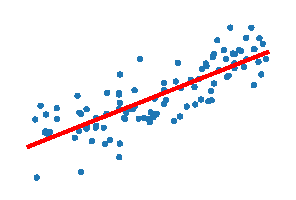
\includegraphics{linear_regression}}
        \end{column}
    \end{columns}
\end{frame}

\begin{frame}
    \frametitle{A (much) more complicated example}
    \begin{columns}
        \begin{column}{0.37\textwidth}
            \begin{block}{Image classification}
                A canonical problem: given an image, predict the correct label
            \end{block}
        \end{column}
        \begin{column}{0.63\textwidth}
            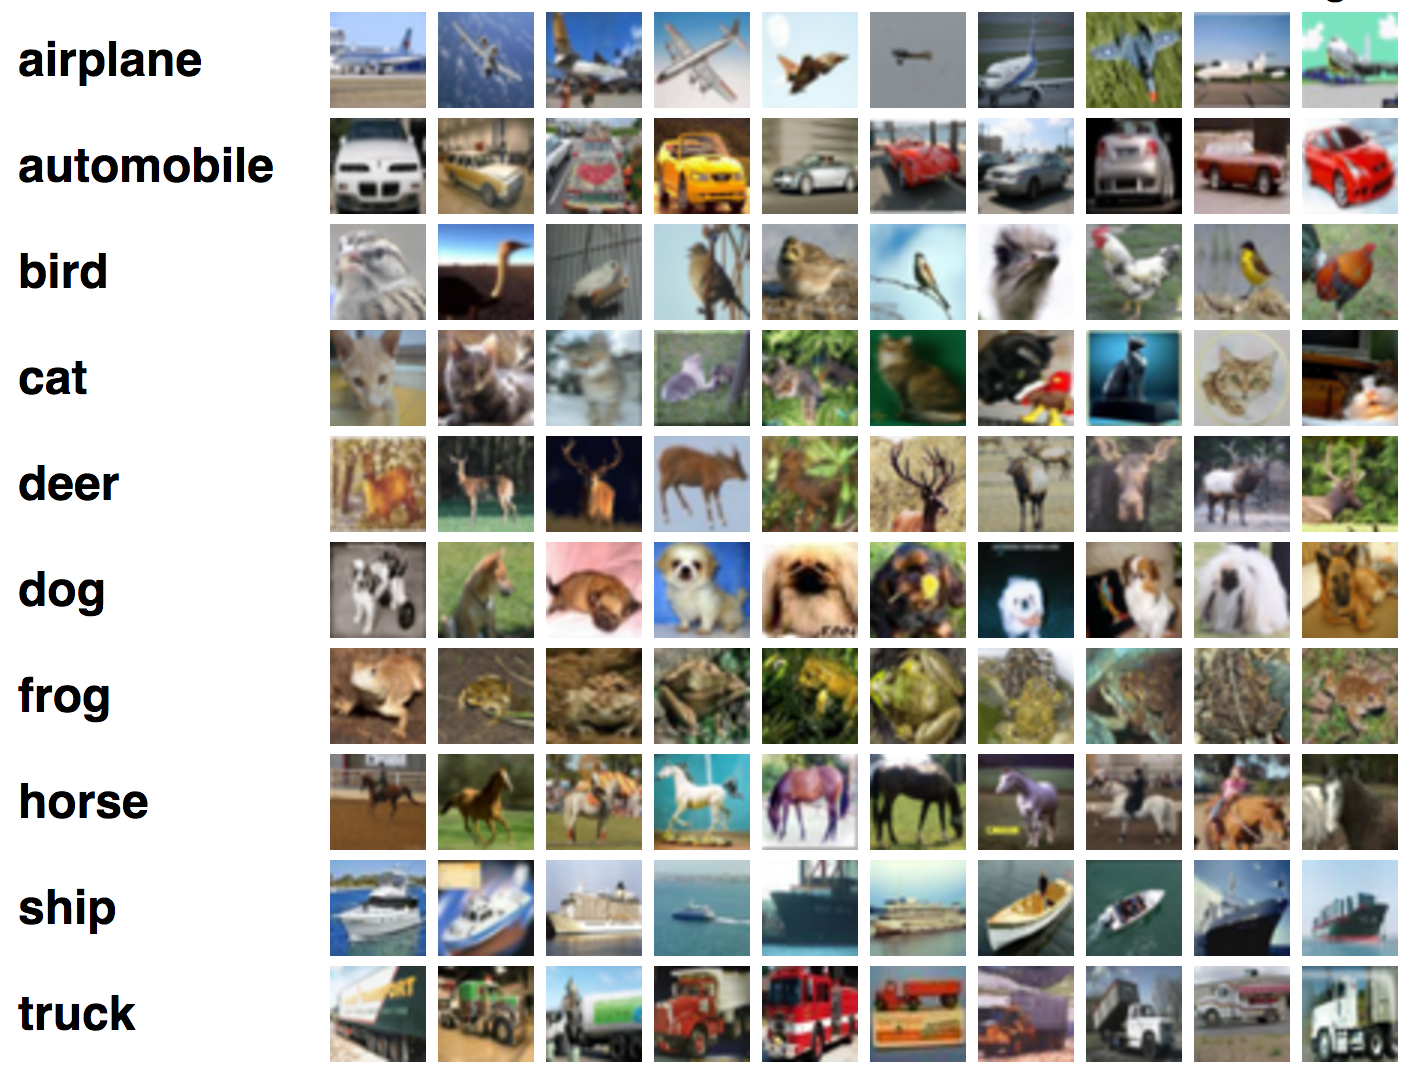
\includegraphics[width=\textwidth]{cifar10} \\
            \centering \footnotesize The CIFAR-10 problem
        \end{column}
    \end{columns}

    \begin{itemize}
        \item Roughly: if a human can do it, a computer should be able to too
        \item More rigorously: $\exists$ a mapping from image pixels to labels
        \begin{itemize}
            \item Mapping too difficult for humans to understand
            \item Let an algorithm model it
        \end{itemize}
    \end{itemize}
\end{frame}

\begin{frame}
    \frametitle{An image classification solution}

    \begin{columns}
        \begin{column}{0.7\textwidth}
            ResNet-152: a 152-layer convolutional neural network with 11.3 billion multiply/adds! \citep{He15b}
            \begin{itemize}
                \item Trained on ImageNet data: 14,197,122 images
                \item Iterative training
                \begin{itemize}
                    \item 600,000 training iterations
                    \item At each iteration, model parameters updated based on \emph{mini-batch} of 256 images
                \end{itemize}
                \item Won multiple image classification competitions
            \end{itemize}
        \end{column}
        \begin{column}{0.3\textwidth}
            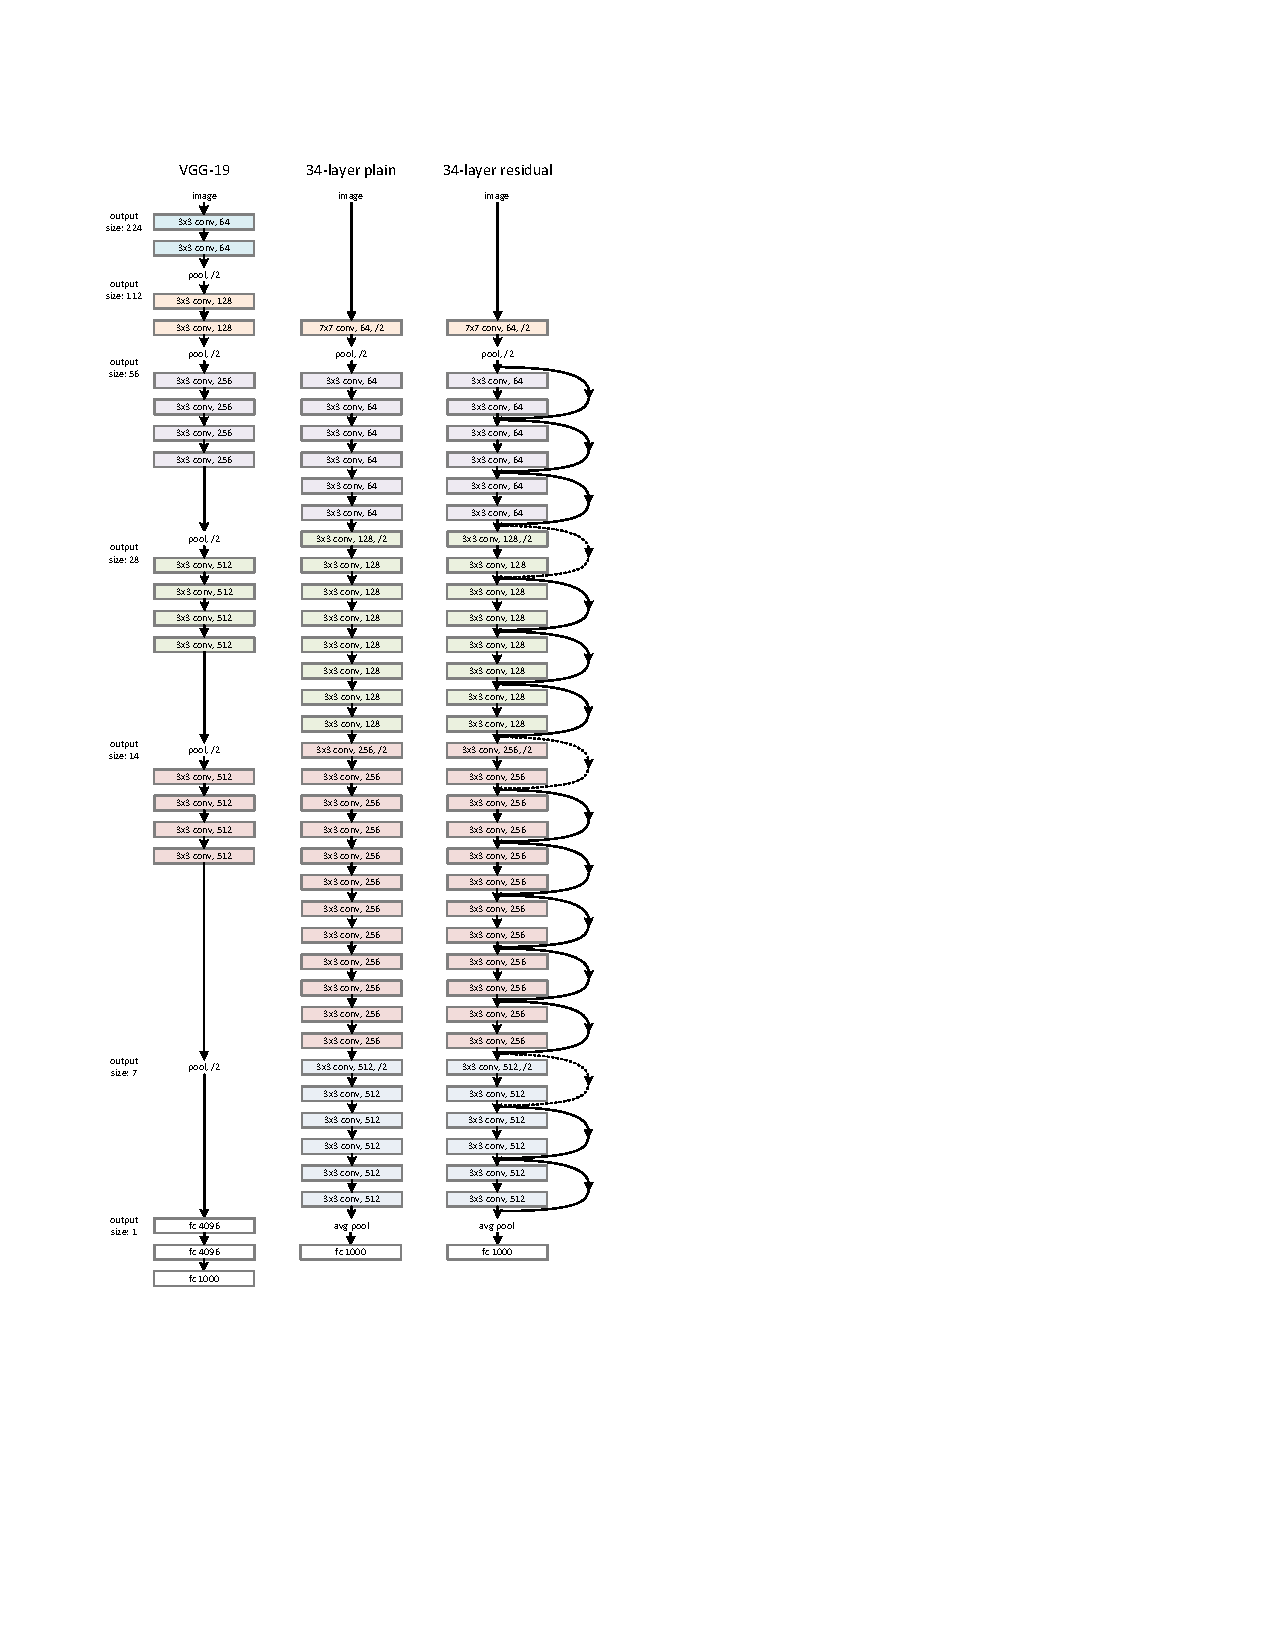
\includegraphics[width=\textwidth]{resnet}
        \end{column}
    \end{columns}
\end{frame}

\begin{frame}
    \frametitle{Supervised learning}
    Machine learning problems/algorithms categorized as \alert{supervised} vs.\ \alert{unsupervised}

    \begin{block}{Supervised learning}
        \begin{itemize}
            \item Data represented as $\{(\x_i, \y_i)\}_{i=1}^n$, with $\x_i$ an input (called \alert{features} or a \alert{feature vector}) and $\y_i$ an output
            \item Given $\x$, predict $\y$
        \end{itemize}
    \end{block}
    \pause

    Supervised learning further split into: \\[1ex]
    \begin{columns}[t]
        \begin{column}{0.47\textwidth}
            \alert{Regression}: $\y$ continuous, e.g.
            \begin{itemize}
                \item $\x =$ (age, sex, race, weight, height, LDL, HDL, zip code, etc.), $y =$ life expectancy
                \item $\x =$ (stock price history, market conditions, interest rates, etc.), $y =$ tomorrow's stock price
            \end{itemize}
        \end{column}
        \pause
        \begin{column}{0.45\textwidth}
            \alert{Classification}: $\y$ discrete, e.g.
            \begin{itemize}
                \item $\x =$ lots of pixels, $\y =$ image label (cat, dog, etc.)
            \end{itemize}
        \end{column}
    \end{columns}
\end{frame}

\begin{frame}
    \frametitle{More supervised learning examples}

    Regression
    \begin{itemize}
        \item Text-to-speech: $\x =$ words, $\y =$ speech audio
        \item Denoising: $\x = \text{data} + \text{noise}$, $\y = \text{data}$
        \item Anomaly detection: $\x =$ (time, location, amount, type) of credit card purchase, $y = \Prob(\text{fraud})$
        \item Prognosis: $\x =$ conditions of existing medical condition, $y =$ expected remaining life
    \end{itemize}
    \pause

    Classification
    \begin{itemize}
        \item Speech-to-text: $\x =$ audio speech sample, $\y =$ words spoken
        \item Spell check: $\x =$ misspelled word, $\y =$ intended word
        \item Machine translation: $\x =$ a sentence in English, $\y =$ the sentence in French
        \item Recommender problem: $\x =$ list of movies you like/dislike, $y =$ whether you like \emph{Interstellar}
        \item Diagnosis: $\x =$ your complete medical record, $\y =$ what medical condition(s) you have
    \end{itemize}
\end{frame}

\begin{frame}
    \frametitle{Converting classification to regression: one-hot}

    Classification problems almost always converted to regression via easy trick

    \begin{block}{One-hot encoding}
        For labels $1, \dots, n$, represent each label as the unit vector $\e_i$, $i = 1, \dots, n$ \\[1ex]
    \end{block}
    \pause

    One-hot vectors loosely interpreted as
    \begin{equation*}
        \begin{bmatrix}
            \Prob(\text{label} = 1) & \cdots & \Prob(\text{label} = n)
        \end{bmatrix}
    \end{equation*}

    E.g. image classification: \\[0.5ex]

    \centering
    \begin{tabular}{c|cc}
        label & index & one-hot vector \\
        \hline
        bird & 1 & $\begin{bmatrix} 1 & 0 & 0 & 0 & \cdots & 0 \end{bmatrix}$ \\
        cat & 2 & $\begin{bmatrix} 0 & 1 & 0 & 0 & \cdots & 0 \end{bmatrix}$ \\
        dog & 3 & $\begin{bmatrix} 0 & 0 & 1 & 0 & \cdots & 0 \end{bmatrix}$ \\
    \end{tabular}
\end{frame}

\begin{frame}
    \frametitle{Converting classification to regression: softmax}
    One-hot works for labeling data.
    What about model outputs?

    \begin{block}{Softmax activation}
        Converts arbitrary real vector (called \textcolor{blue}{logits}) to \textcolor{Green4}{vector of probabilities that sums to 1}
        \vspace{-1pt}
        \begin{align*}
            \softmax &: \textcolor{blue}{\Reals^n} \to
            \textcolor{Green4}{(0, 1)^n \text{ with } L^1 \text{ norm} = 1} \\
            &\hspace{1.25ex} \textcolor{blue}{%
                \left(\begin{bmatrix} y_1 & \cdots & y_n \end{bmatrix}\right)%
            } \mapsto
            \textcolor{Green4}{%
                \frac{1}{\sum_{i=1}^n e^{y_i}}
                \begin{bmatrix}
                    e^{y_1} & \cdots & e^{y_n}
                \end{bmatrix}%
            }
        \end{align*}
        \vspace{-10pt}
    \end{block}
    \pause

    Like one-hot, output loosely interpreted as
    \begin{equation*}
        \textcolor{Green4}{%
            \begin{bmatrix}
                \Prob(\text{label} = 1) & \cdots & \Prob(\text{label} = n)
            \end{bmatrix}
        }
    \end{equation*}
    (Real statisticians object to calling these \emph{probabilities}; we'll be flexible)

    \begin{itemize}
        \item E.g.: model outputs \textcolor{blue}{%
            logits
            $\y = \begin{bmatrix} -3.33 & 9.62 & 9.18 & \cdots \end{bmatrix}$
        }
        \item \textcolor{Green4}{%
            $\softmax(\y) = \begin{bmatrix} 1.40 \cdot 10^{-6} & 0.593 & 0.381 & \cdots \end{bmatrix}$
        }
        \item Model is 59.3\% confident in ``cat,'' 38.1\% confident in ``dog''
    \end{itemize}
\end{frame}

\begin{frame}
    \frametitle{Converting classification to regression: sigmoid}
    If $\exists$ only two classes (e.g., yes/no), second probability is redundant.
    Alternative:

    \begin{columns}
        \begin{column}{2.3in}
            \begin{block}{Standard logistic activation}
                Converts arbitrary real scalar (called \textcolor{blue}{logit}) to single probability
                \begin{align*}
                    \sigma &: \textcolor{blue}{\Reals} \to \textcolor{Green4}{(0, 1)} \\
                    &\hspace{1.25ex} \textcolor{blue}{y} \mapsto
                    \textcolor{Green4}{\frac{1}{1 + e^{-y}}}
                \end{align*}
            \end{block}
        \end{column}
        \begin{column}{1.8in}
            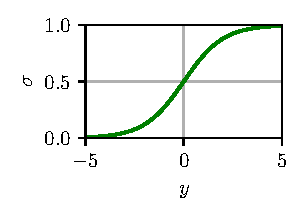
\includegraphics{sigmoid}
        \end{column}
    \end{columns}
    \vspace{1em}
    \pause

    Loose interpretation: $\Prob(\text{yes}) = \sigma(y)$, $\Prob(\text{no}) = 1 - \sigma(y)$

    \begin{itemize}
        \item Technically, any function of this shape is called ``sigmoid''
        \item Many people use ``sigmoid'' to refer specifically to the standard logistic
    \end{itemize}
\end{frame}

\begin{frame}[t]
    \frametitle{Unsupervised learning}
    \begin{block}{Unsupervised learning}
        \begin{itemize}
            \item Data represented as $\{x_i\}_{i=1}^n$ only: no outputs
            \item \alert{Density estimation}: learn the data's probability distribution
        \end{itemize}
    \end{block}

    \uncover<2->{Related problem: \alert{clustering}---find which clusters data belong to} \\[1ex]

    \uncover<4->{Examples:}
    \begin{itemize}
        \item<4-> Generative modeling: given \textcolor<5->{blue}{pictures of volcanoes}, generate \textcolor<5->{Green4}{new ones that look realistic}
        \item<6-> Determine if loan/insurance applicant is low/medium/high-risk
    \end{itemize}

    \temporal<2>{%
    }{%
        
\includegraphics{cluster}%
    }{%
        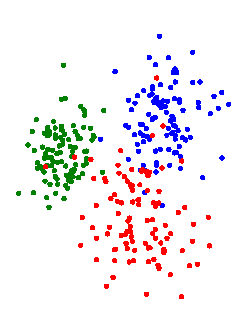
\includegraphics{clusters}%
    }
    \hfill
    \begin{tikzpicture}[
        node distance=5mm,
        frame/.style={draw, rectangle, ultra thick, inner sep=1pt}
    ]
        \visible<4->{
            \node (real) [frame, temporal=<5>{white}{blue}{blue}] {
                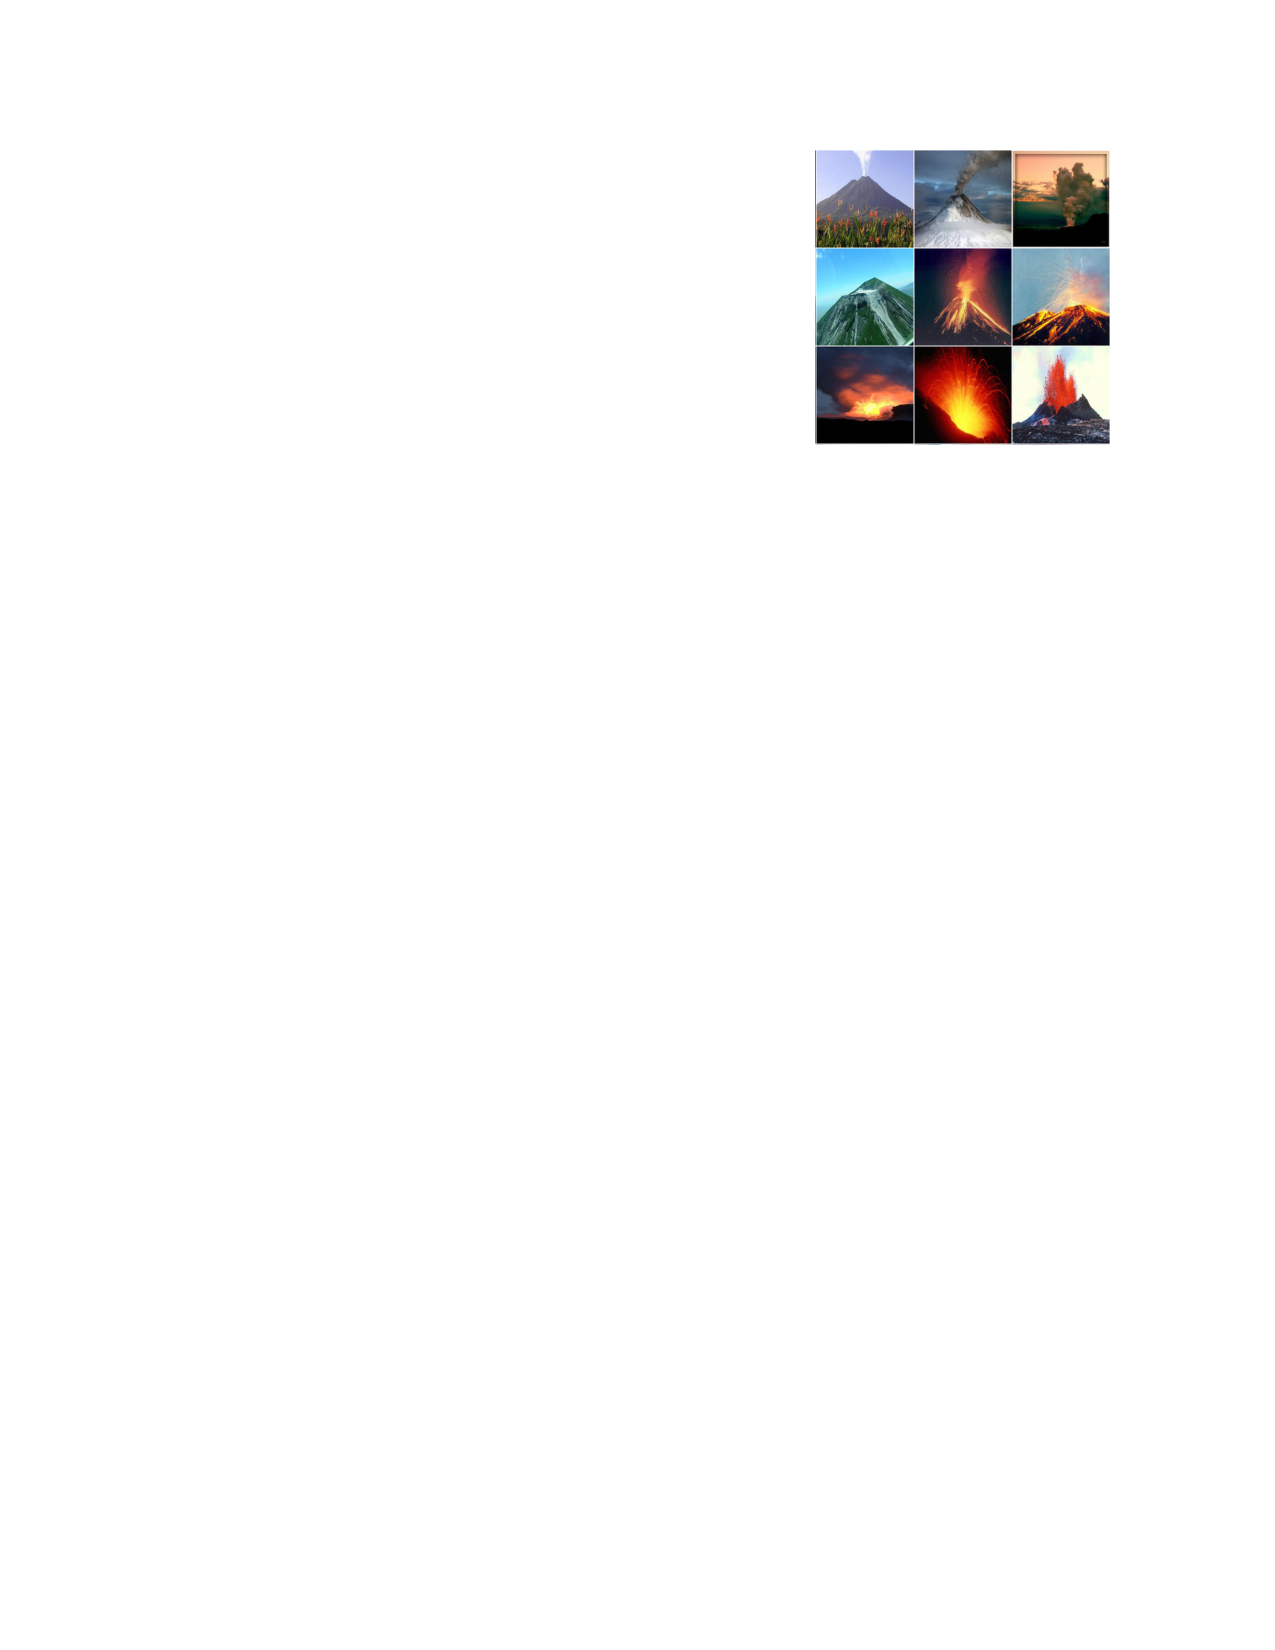
\includegraphics[width=3.2cm]{volcano_data}
            };
            \node (gen) [right=of real, frame, temporal=<5>{white}{Green4}{Green4}] {
                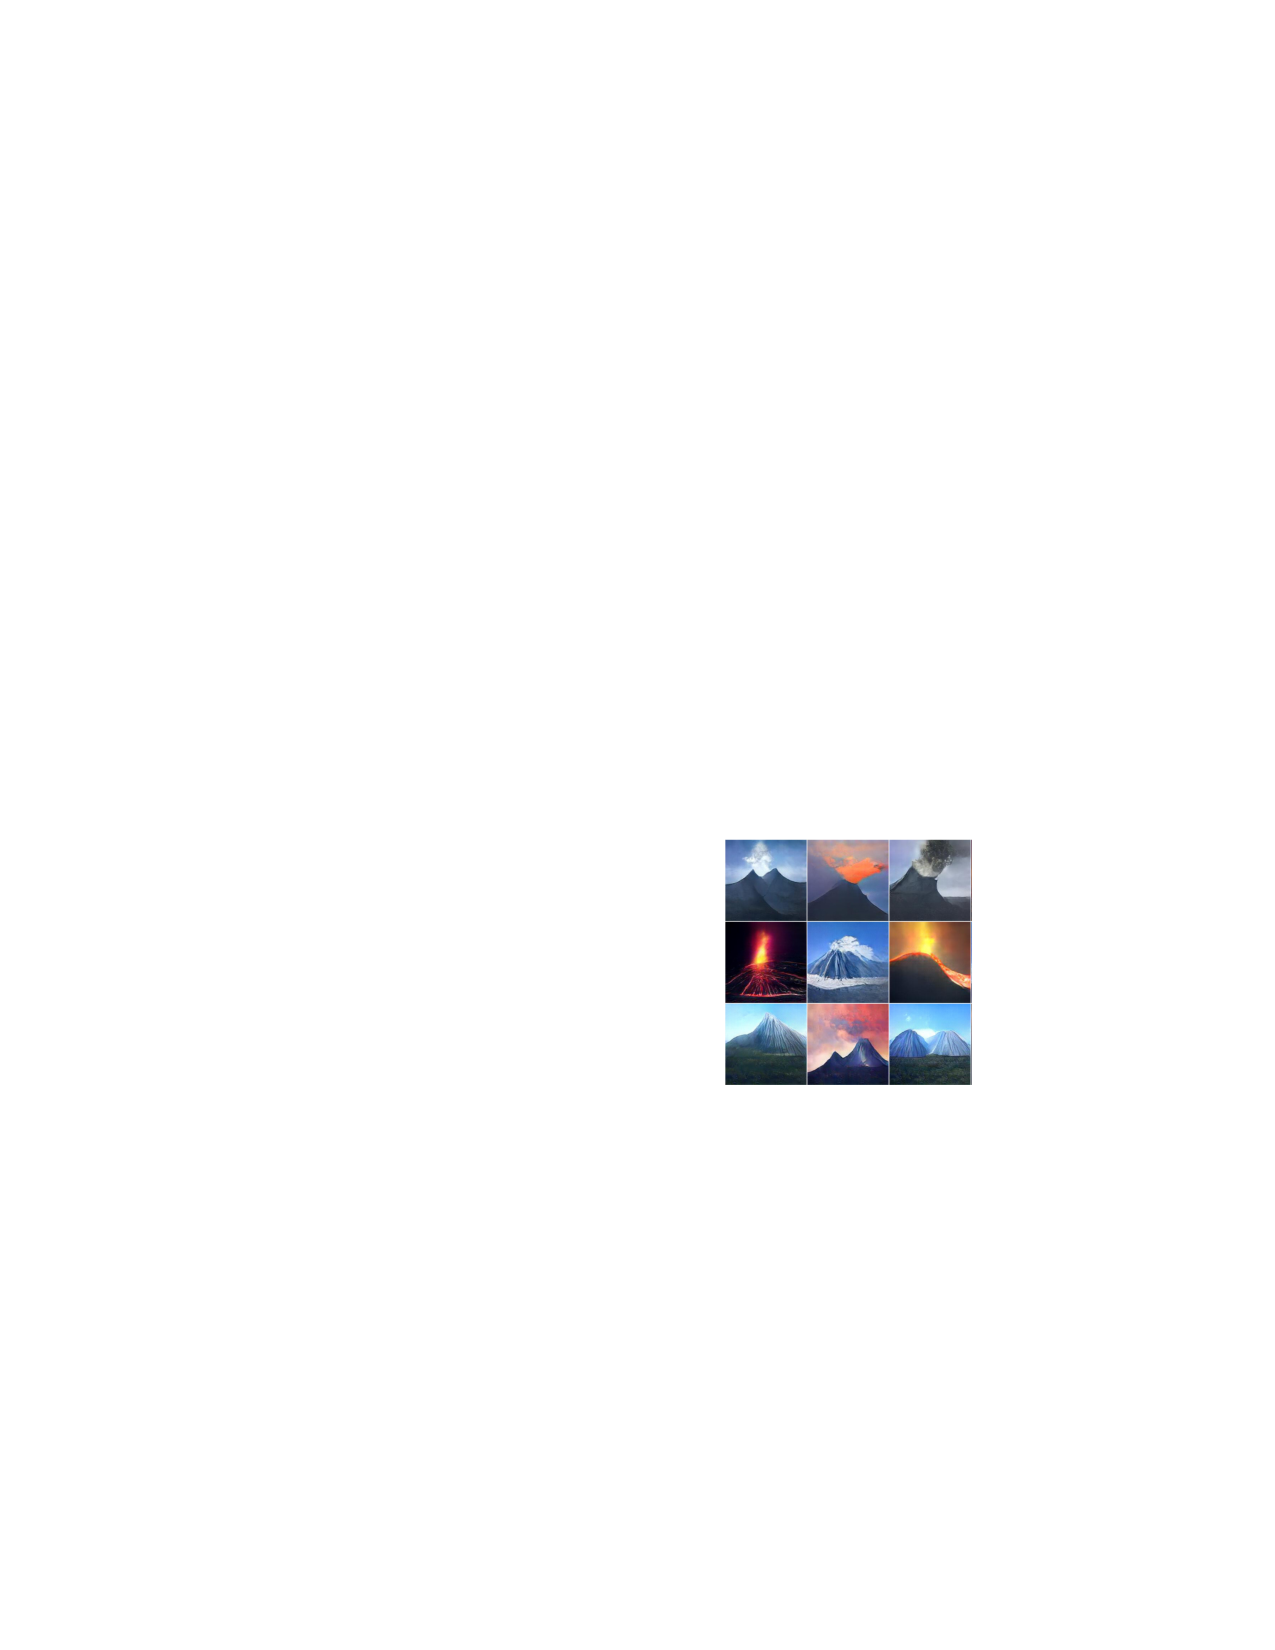
\includegraphics[width=3.2cm]{volcano_generated}
            };
        }
    \end{tikzpicture}
\end{frame}

\begin{frame}
    \frametitle{Notes on supervised vs.\ unsupervised learning}

    \begin{itemize}
        \item I will only focus on supervised learning today \& Thursday
        \begin{itemize}
            \item Theory more mature
            \item Techniques more powerful
        \end{itemize}
        \item Many experts believe a strong future in ML requires a shift toward unsupervised learning
        \begin{itemize}
            \item $\exists$ tons of data in the world, but mostly unlabeled
        \end{itemize}
        \item Semi-supervised learning: usually, small amount of labeled data + lots of unlabeled data
    \end{itemize}
\end{frame}

\begin{frame}
    \frametitle{Machine learning algorithms}

    \begin{columns}
        \begin{column}{0.44\textwidth}
            The list is long:
            \begin{itemize}[<.->]
                \item Logistic regression
                \item Gaussian mixture models
                \item Kernel methods
                \item Naive Bayes classifier
                \item $k$-nearest neighbors, $k$-means, $k$-medians
                \item Decision trees
                \item Random forests
                \item Support vector machines
                \item \alert<2->{(Artificial) neural networks}
                \item Etc.
            \end{itemize}
        \end{column}

        \begin{column}{0.56\textwidth}
            \uncover<2->{%
                I will only focus on neural networks.
                Even then, variations are plentiful:
            }
            \begin{itemize}[<2->]
                \item \alert<3->{Dense (fully-connected) NN: generic}
                \item Convolutional NN: for spatial data
                \item \alert<3->{Recurrent NN: for temporal data (Thursday's topic)}
                \item Autoencoders: for data representations
                \item Reinforcement learning: for AI/games
                \item Generative models: for making new data
                \item Recommender systems
                \item Etc.
            \end{itemize}
            \uncover<2->{These can generally be combined freely}
        \end{column}
    \end{columns}
\end{frame}

%%% Local Variables:
%%% mode: latex
%%% TeX-master: "../nn"
%%% End:

\section{Loss}

\subsection{}

\begin{frame}
    \frametitle{How good is a prediction?}

    \begin{itemize}
        \item $\x \in \X$: data \& model input
        \item $\y \in \Y$: data output
        \item $\yh \in \Yh$: model output with $\dim(\Yh) = \dim(\Y)$ (generally, $\Yh = \Y$)
        \item $\f : \X \to \Yh, \x \mapsto \yh$: model
    \end{itemize}
    \pause

    \begin{block}{Loss function}
        A function that specifies how bad of a prediction $\yh = \f(\x)$ is for the ground truth $\y$
        \begin{equation*}
            L : \Y \times \Yh \to \Reals_{\ge 0}
        \end{equation*}
    \end{block}
    \pause

    We will see that ``training a machine learning algorithm'' basically means ``minimizing the expected loss over the training data.'' \\[1ex]

    You get to pick the loss function!
\end{frame}

\begin{frame}
    \frametitle{Regression loss functions}
    Let $\y = \begin{bmatrix} y_1 & \cdots & y_n \end{bmatrix}$,
    $\yh = \begin{bmatrix} \hat{y}_1 & \cdots & \hat{y}_n \end{bmatrix}$

    \begin{block}{Mean squared error}
        \vspace{-1em}
        \begin{align*}
            L(\y, \yh) &:= \frac{1}{n} \sum_{i=1}^n (y_n - \hat{y}_n)^2 \\
            &= \dfrac{\|\y - \yh\|_2^2}{n}
        \end{align*}
        \vspace{-1em}
        \begin{itemize}
            \item Most common loss for regression
        \end{itemize}
    \end{block}
    \pause

    \begin{block}{Mean absolute error}
        \vspace{-1em}
        \begin{align*}
            L(\y, \yh) &:= \frac{1}{n} \sum_{i=1}^n |y_n - \hat{y}_n| \\
            &= \dfrac{\|\y - \yh\|_1}{n}
        \end{align*}
        \vspace{-1em}
    \end{block}
\end{frame}

\begin{frame}
    \frametitle{Classification loss functions}
    Assumptions:
    \begin{itemize}
        \item<+-> correct label $= k$; $\y = \e_k$ (one-hot)
        \item<.-> $\yh =
        \begin{bmatrix}
            \hat{y}_1 & \cdots & \hat{y}_n
        \end{bmatrix} =
        \begin{bmatrix}
            \Prob(\text{label} = 1) & \cdots & \Prob(\text{label} = n)
        \end{bmatrix}$
    \end{itemize}

    \begin{block}{Zero--one loss}<+->
        \begin{equation*}
            L(\y, \yh) := \begin{cases}
                0 &\mid \argmax(\yh) = k \\
                1 &\mid \argmax(\yh) \ne k
            \end{cases}
        \end{equation*}
        \begin{itemize}
            \item Easiest, but non-differentiable
        \end{itemize}
    \end{block}

    \begin{block}{(Categorical) cross-entropy loss}<+->
        \begin{equation*}
            L(\y, \yh) := -\log\hat{y}_k = \log\left(\dfrac{1}{\Prob(\text{label} = k)}\right)
        \end{equation*}
        \begin{itemize}
            \item Most common loss for labeling with $> 2$ classes
            \item $L = 0 \iff P(\text{label} = k) = 1$;
            $L \to \infty \iff P(\text{label} = k) \to 0$
        \end{itemize}
    \end{block}
\end{frame}

\begin{frame}
    \frametitle{Classification loss function: more cross-entropy}
    Recall: for binary problems, classes are $y = 0$ (no) and $1$ (yes)

    \begin{block}{Binary cross-entropy loss}
        \vspace{-1em}
        \begin{align*}
            L(y, \hat{y}) &:= -y \log \hat{y} - (1 - y) \log(1 - \hat{y}) \\
            &= \begin{cases}
                -\log(1 - \hat{y}) &\mid y = 0 \\
                -\log \hat{y} &\mid y = 1
            \end{cases}
        \end{align*}
    \end{block}
    \pause

    Note: high accuracy $\centernot\implies$ small loss
    \begin{itemize}
        \item Typically, model prediction taken to be $\argmax(\yh)$
        \item Cross-entropy penalizes being unconfident about correct label, \emph{not} having the wrong $\argmax(\yh)$
        \pause
        \item E.g., if $k = 3$ is correct answer, cross-entropy:
        \begin{align*}
            L(
                \begin{bmatrix} 0 & 0 & 1 & 0 \end{bmatrix},
                \begin{bmatrix}
                    0.05 & 0.03 & \textcolor{blue}{0.9} & 0.02
                \end{bmatrix}
            ) &= 0.105 \\
            L(
                \begin{bmatrix} 0 & 0 & 1 & 0 \end{bmatrix},
                \begin{bmatrix}
                    0.25 & 0.25 & \textcolor{blue}{0.26} & 0.24
                \end{bmatrix}
            ) &= 1.35
        \end{align*}
        even though both $\yh$ correctly predict $\argmax(\yh) = 3$
    \end{itemize}
\end{frame}

\begin{frame}
    \frametitle{Model risk and batch loss}

    The \alert{model risk} is the expected loss over all $\x \in \X$ with distribution $p_\X$:

    \begin{block}{Model risk}
        \vspace{-1em}
        \begin{align*}
            R(\f) &:= \E_{\x \sim p_\X}(\E_{\y \mid \x}(L(\y, \f(\x)))) \\
            &= \int_\X \int_\Y L(\y, \f(\x)) \Prob(\y | \x) \, \dy \Prob(\x) \, \dx
        \end{align*}
    \end{block}
    \pause

    Since we usually can't exhaust over all $\x \in \X$, select a batch $\S = \{(\x_i, \y_i)\}_{i=1}^m \subset \X \times \Y$, then use:

    \begin{block}{Approximate model risk / batch loss}
        \vspace{-1em}
        \begin{align*}
            \hat{R}(\f) &:= \E_{(\x, \y) \in \S}(L(\y, \f(\x))) \\
            &= \frac{1}{m} \sum_{i=1}^m L(\y_i, \f(\x_i))
        \end{align*}
    \end{block}
    \pause

    Objective of ML training: \alert{minimize $\hat{R}$ over some data set}
    \begin{itemize}
        \item From now on I'll just call it $R$
    \end{itemize}
\end{frame}

%%% Local Variables:
%%% mode: latex
%%% TeX-master: "../nn"
%%% End:

\section{Dense neural networks}

\subsection{}

\begin{frame}
    \frametitle{The neuron: equations}

    Consider an input $\x \in \Reals^q$.
    \begin{block}{}
        Consider some \emph{weight vector} $\w \in \Reals^q$ and \emph{bias} $b \in \Reals$.
        The mapping
        \begin{align*}
            g &: \Reals^q \to \Reals \\
            &\hspace{1.25ex} \x \mapsto \w \cdot \x + b
        \end{align*}
        is an \alert{affine transformation}.
    \end{block}
    \pause

    Consider a generally nonlinear \alert{activation function} $\sigma: \Reals \to \Reals$.

    \begin{block}{}
        An (artifical) \alert{neuron} is the function $\phi = \sigma \circ g$, i.e.,
        \begin{align*}
            \phi &: \Reals^q \to \Reals \\
            &\hspace{1.25ex} \x \mapsto \sigma(\w \cdot \x + b)
        \end{align*}
    \end{block}
    \pause

    \begin{itemize}
        \item Historically, artificial neuron modeled on biological neurons
        \begin{itemize}
            \item Bio neuron triggers impulse by nonlinear function of inputs
        \end{itemize}
        \item Today, relation is largely only conceptual/philosophical
    \end{itemize}
\end{frame}

\begin{frame}
    \frametitle{The neuron: geometric interpretation}
\end{frame}

\begin{frame}
    \frametitle{Single hidden-layer neural network: vector equations}

    Consider $n$ neurons each taking in $\x \in \Reals^q$: given
    \begin{itemize}
        \item weight vectors $\w_k \in \Reals^q$, $k = 1, \ldots, n$,
        \item biases $b_k \in \Reals$, $k = 1, \ldots, n$,
    \end{itemize}
    \begin{block}{Hidden layer}
        \vspace{-1em}
        \begin{align*}
            z_k &= \sigma(\w_k \cdot \x + b_k), \quad k = 1, \ldots, n \\
            \z &= \begin{bmatrix} z_1 & \cdots & z_n \end{bmatrix} \in \Reals^n
        \end{align*}
    \end{block}
    \pause

    Let the model output $\y \in \Reals^p$ be affine transformations of $\z$: given
    \begin{itemize}
        \item weight vectors $\v_k \in \Reals^n$, $k = 1, \ldots, p$
        \item biases $c_k \in \Reals$, $k = 1, \ldots, p$
    \end{itemize}
    \begin{block}{Single hidden-layer neural network}
        \vspace{-1em}
        \begin{align*}
            y_k &= \v_k \cdot \z + c_k, \quad k = 1, \ldots, p \\
            \y &= \begin{bmatrix} y_1 & \cdots & y_p \end{bmatrix}
        \end{align*}
    \end{block}
\end{frame}

\begin{frame}
    \frametitle{Single hidden-layer neural network: figure}

    \centering
    \begin{tikzpicture}[>=latex, node distance=9mm]
    % Inputs.
    \uncover<+->{
        \node (x1) [scalar] {$x_1$};
        \node (x2) [scalar, right=of x1] {$x_2$};
        \node (x3) [scalar, right=of x2] {$\cdots$};
        \node (x4) [scalar, right=of x3] {$x_q$};

        \node [right=1.25cm of x4] {$\x$};

    }

    \uncover<+->{
        % Hidden layer.
        \draw [very thick, rounded corners, fill=red!10]
        (-1.2, 0.9) rectangle (6.27, 3.5);

        % Hidden layer combinations.
        \node (affine x1) [affine, above=of x1, xshift=-5mm] {affine};
        \node (affine x2) [affine, right=6mm of affine x1] {affine};
        \node (affine x3) [affine, right=6mm of affine x2] {affine};
        \node (affine x4) [affine, right=6mm of affine x3] {$\cdots$};
        \node (affine x5) [affine, right=6mm of affine x4] {affine};

        \node [right=4.3mm of affine x5] {$\w_k \cdot \x + b_k$};
    }

    \uncover<+->{
        % Hidden layer activations.
        \foreach \i in {1, 2, 3, 5} {
            \node (sigma\i) [activation, above=4mm of affine x\i] {$\sigma$};
        }

        \node (sigma4) [activation, above=4mm of affine x4] {$\cdots$};

        \node [right=5.5mm of sigma5] {$z_k = \sigma(\w_k \cdot \x + b_k)$};
    }

    % Output combinations.
    \uncover<+->{
        \node (affine y1) [affine, above=of sigma2] {affine};
        \node (affine y2) [affine, above=of sigma3] {$\cdots$};
        \node (affine y3) [affine, above=of sigma4] {affine};

        \node [right=1.88cm of affine y3] {$y_k = \v_k \cdot \z + c_k$};
    }

    % Outputs.
    \uncover<+->{
        \node (y1) [scalar, above=of affine y1] {$y_1$};
        \node (y2) [scalar, above=of affine y2] {$\cdots$};
        \node (y3) [scalar, above=of affine y3] {$y_p$};

        \node [right=2cm of y3] {$\y$};
    }

    % Connections.

    \foreach \i/\a in {1/130, 2/110, 3/90, 4/70, 5/50} {
        % Inputs to affines.
        \foreach \j/\b in {1/230, 2/257, 3/283, 4/310} {
            \uncover<2->{\draw [path] (x\j.\a) -- (affine x\i.\b);}
        }

        % Hidden layer affines to activations.
        \uncover<3->{\draw [path] (affine x\i) -- (sigma\i);}
    }

    \foreach \j/\b in {1/120, 2/90, 3/60} {
        % Hidden layer activations to output affines.
        \foreach \i/\a in {1/230, 2/250, 3/270, 4/290, 5/310} {
            \uncover<4->{\draw [path] (sigma\i.\b) -- (affine y\j.\a);}
        }

        % Output affines to outputs.
        \uncover<5->{\draw [path] (affine y\j) -- (y\j);}
    }
\end{tikzpicture}

%%% Local Variables:
%%% mode: latex
%%% TeX-master: "../nn"
%%% End:

\end{frame}

\begin{frame}
    \frametitle{Single hidden-layer neural network: matrix equations}

    The equations are more compact in matrix form:
    \begin{itemize}
        \item Weight matrix $\W \in \Reals^{n \times q}$
        \item Bias vector $\b \in \Reals^n$
        \item Element-wise activation function
        \begin{align*}
            \SIGMA &: \Reals^n \to \Reals^n \\
            &\hspace{1.25ex} \begin{bmatrix} \xi_1 & \cdots & \xi_n \end{bmatrix} \mapsto
            \begin{bmatrix} \sigma(\xi_1) & \cdots & \sigma(\xi_n) \end{bmatrix}
        \end{align*}
    \end{itemize}

    \begin{block}{Hidden layer}
        \begin{equation*}
            \z = \SIGMA(\W \x + \b)
        \end{equation*}
    \end{block}
    \pause

    \begin{itemize}
        \item Weight matrix $\V \in \Reals^{q \times n}$
        \item Bias vector $\c \in \Reals^q$
    \end{itemize}

    \begin{block}{Single hidden-layer neural network}
        \begin{equation*}
            \y = \V \z + \c
        \end{equation*}
    \end{block}
\end{frame}

\begin{frame}
    \frametitle{Activation functions}
    \begin{block}{Why do neurons have nonlinear activation functions?}
        If $\sigma$ is linear (including the identity $\sigma(x) = x$, i.e. no activation), the neural network $\f : \x \mapsto \y$ is necessarily linear \\[1ex]
        For $\f$ to be nonlinear, \alert{activation functions must be nonlinear}!
    \end{block}

    In some sense, it doesn't even matter what $\sigma$ is, as long as it's nonlinear. \\[1ex]

    To be more particular, $\sigma$ should
    \begin{itemize}
        \item be fast to compute (will be called gazillions of times)
        \item not lead to vanishing or exploding gradients
    \end{itemize}
\end{frame}

\begin{frame}
    \frametitle{Common activation functions}
    \begin{columns}
        \begin{column}{2.5in}
            \begin{itemize}
                \item \textcolor{Green4}{Standard logistic/sigmoid function: $\sigma(x) = \dfrac{1}{1 + e^{-x}} = \dfrac{\tanh(x) + 1}{2}$}
                \begin{itemize}
                    \item Used to be preferred
                    \item Now thought to be too slow
                    \item Suffers from vanishing gradients
                \end{itemize}
                \item \textcolor{blue}{Rectified linear unit (ReLU): $\sigma(x) = \max(0, x)$}
                \begin{itemize}
                    \item Most common, but suffers from vanishing gradients
                \end{itemize}
                \item \textcolor{red}{Leaky/parametric ReLU \citep{MaasICML13}: $\sigma(x) = \begin{cases} x &\mid x \ge 0 \\ \alpha x &| x < 0 \end{cases}$}
                \item \textcolor{magenta}{Exponential linear unit (ELU) \citep{ClevertICLR16}: $\sigma(x) = \begin{cases} x &\mid x > 0 \\ \alpha (e^x - 1) &\mid x \le 0 \end{cases}$}
            \end{itemize}
        \end{column}
        \begin{column}{2in}
            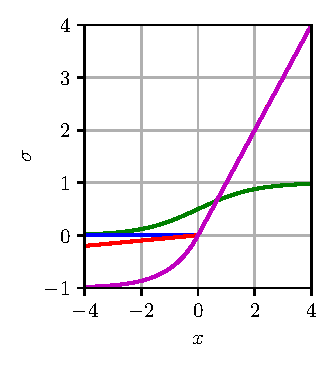
\includegraphics{activations}
        \end{column}
    \end{columns}
\end{frame}

\begin{frame}
    \frametitle{Deep neural networks}

    No reason to stop at only one hidden layer!

    \vspace{1mm}
    \begin{tikzpicture}[node distance=6mm]
    % Layer 1.
    \uncover<2->{\node (n11) [neuron] {};}

    \foreach \i in {1, ..., 4} {
        \pgfmathtruncatemacro{\j}{\i + 1}
        \uncover<2->{\node (n1\j) [neuron, right=of n1\i] {};}

        % Inputs.
        \node (x\i) [io, below=of n1\i, xshift=6mm] {};
        % Layer 2.
        \uncover<3->{\node (n2\i) [neuron, above=of n1\i, xshift=6mm] {};}
    }

    \foreach \i in {1, ..., 3} {
        % Invisible layer 3.
        \node (n3\i) [minimum width=5mm, above=of n2\i, xshift=5mm] {};
        % Invisible layer 4.
        \node (n4\i) [above=4mm of n3\i] {};
    }

    % Etc.
    \uncover<4->{\node (etc) [above=8mm of n22, xshift=6mm] {$\vdots$};}

    \uncover<5->{
        \node (nl1) [neuron, above=of etc, xshift=-6mm] {};
        \node (nl2) [neuron, right=of nl1] {};
    }

    % Outputs.
    \uncover<6->{
        \node (y2) [io, above=of nl1] {};
        \node (y3) [io, above=of nl2] {};
        \node (y1) [io, left=of y2] {};
        \node (y4) [io, right=of y3] {};
    }

    \node [right=of x4, xshift=5.5mm] {$\x \in \Reals^q$};
    \uncover<2->{
        \node [right=of n15] {$\z_1 = \SIGMA(\W_1 \x + \b_1) \in \Reals^{n_1}$};
    }
    \uncover<3->{
        \node [right=of n24, xshift=5.4mm] {$\z_2 = \SIGMA(\W_2 \z_1 + \b_2) \in \Reals^{n_2}$};
    }
    \uncover<4->{
        \node [right=of n33, yshift=-2mm, xshift=1.64cm] {$\vdots$};
        \node [right=of etc, yshift=-1mm, xshift=2.28cm] {$\z_i = \SIGMA(\W_i \z_{i-1} + \b_i) \in \Reals^{n_i}$};
    }
    \uncover<5->{
        \node [right=of n43, yshift=5mm, xshift=1.76cm] {$\vdots$};
        \node [right=of nl2, xshift=1.68cm] {$\z_l = \SIGMA(\W_l \z_{l-1} + \b_l) \in \Reals^{n_l}$};
    }
    \uncover<6->{\node [right=of y4, xshift=5.4mm] {$\y = \V \z_l + \cc \in \Reals^p$};}

    \foreach \i in {1, ..., 4} {
        \foreach \j in {1, ..., 5} {
            \uncover<2->{\draw [path] (x\i.90) -- (n1\j.270);}
            \uncover<3->{\draw [path] (n1\j.90) -- (n2\i.270);}
        }

        \foreach \j in {1, ..., 3} {
            \uncover<4->{\draw [path] (n2\i.90) -- (n3\j.270);}
        }
    }

    \foreach \i in {1, 2} {
        \foreach \j in {1, ..., 3} {
            \uncover<5->{\draw [path] (n4\j.90) -- (nl\i.270);}
        }

        \foreach \j in {1, ..., 4} {
            \uncover<6->{\draw [path] (nl\i.90) -- (y\j.270);}
        }
    }
\end{tikzpicture}

%%% Local Variables:
%%% mode: latex
%%% TeX-master: "../nn"
%%% End:

    \vspace{1mm}

    Common but not necessary for $\SIGMA$ to be the same in each layer
\end{frame}

\begin{frame}
    \frametitle{Why is deep better than wide?}
    \begin{itemize}
        \item Depth: \# layers
        \item Width: \# neurons in each layer (need not be fixed)
    \end{itemize}
    \pause

    Neural network with $\sigma = \text{ReLU}$ is piecewise linear function
    \begin{itemize}
        \item \alert{Expressivity} of ReLU network measured by \# linear pieces
        \item For a network with width $w$ and depth $l$, \alert{$\max \text{expressivity} \sim w^l$} \citep{Pascanu13,MontufarNIPS14,Chen16}
        \begin{itemize}
            \item Polynomial in width
            \item Exponential in depth!
        \end{itemize}
    \end{itemize}
    \pause

    Common for layers closer to the input to be wider
    \begin{itemize}
        \item Closer to the input $\implies$ more expressive power over output \citep{RaghuICML17}
    \end{itemize}
\end{frame}

\begin{frame}
    \frametitle{What can dense neural networks model?}
    % Universal approximation
\end{frame}

%%% Local Variables:
%%% mode: latex
%%% TeX-master: "../nn"
%%% End:


\section{Training}

\subsection{}

% Initialization
% Including train/validation/test, or put in separate section.
% Under/overfit

%%% Local Variables:
%%% mode: latex
%%% TeX-master: "../nn"
%%% End:

\section{Regularization}

\subsection{}

\begin{frame}
    \frametitle{Underfitting and overfitting}

    \begin{alertblock}{Danger!}
        Neural networks are hard to fit, and real-life data are noisy.
        \emph{Underfitting} and \emph{overfitting} are your two biggest obstacles.
    \end{alertblock}
    \vspace{1ex}

    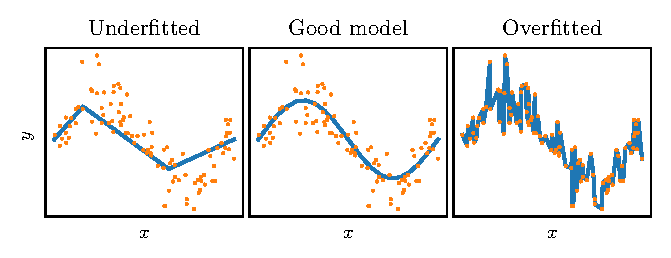
\includegraphics{under_over_train}
    \pause

    \begin{itemize}
        \item Underfitting: didn't train enough for the model to capture the underlying behavior
        \item Overfitting: training so good that neural network memorizes the data, including underlying noise
        \begin{itemize}
            \item Recall: with enough parameters, neural networks learn anything
        \end{itemize}
    \end{itemize}
\end{frame}

\begin{frame}
    \frametitle{Train, validate, test}

    Usual trick: split data into disjoint \textcolor{blue}{training} and \textcolor{Green4}{testing} sets
    \begin{itemize}
        \item Anywhere from 95/5 to 75/25 split is common
        \item Train \emph{only} on the \textcolor{blue}{training set}
        \item Periodically check loss of NN on \textcolor{Green4}{test set}
        \begin{itemize}
            \item Optimizer never sees test set: test set is honest check on NN fidelity
        \end{itemize}
    \end{itemize}
    \pause

    More advanced: split into disjoint \textcolor{blue}{training}, \textcolor{orange}{validation}, and \textcolor{Green4}{testing} set
    \begin{itemize}
        \item Aside on terminology
        \begin{itemize}
            \item Weights \& biases are \alert{parameters}---iteratively improved
            \item Design choices (\# layers, \# neurons, optimizer, \# epochs, etc.) are \alert{hyperparameters}---selected by ML designer
        \end{itemize}
        \item Select different sets of hyperparameters; for each:
        \begin{itemize}
            \item Train only on \textcolor{blue}{training set}, as before
            \item Compute validation loss on \textcolor{orange}{validation set}
        \end{itemize}
        \item Pick hyperparameters with lowest validation loss
        \item Then re-evaluate loss on \textcolor{Green4}{test data}
        \begin{itemize}
            \item Helps remove effects of variance on validation loss
        \end{itemize}
    \end{itemize}
\end{frame}

\begin{frame}
    \frametitle{Training loss vs.~test loss}
    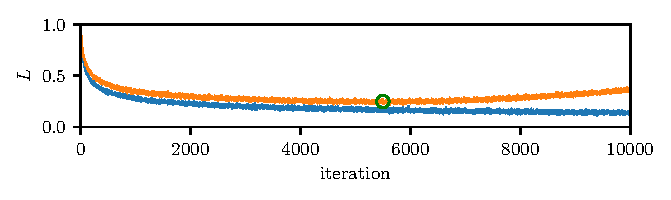
\includegraphics{loss}

    General pattern
    \begin{itemize}
        \item Modulo minor stochastic fluctuations, training loss should monotonically decrease: NN gets better at learning data
        \item Test loss usually at least slightly larger than training loss
        \begin{itemize}
            \item Because optimizer minimizes training loss but never sees test data
        \end{itemize}
        \item At some point, test loss increases: NN overfits to training data
        \item \alert{Early stopping}: use NN with minimum test loss
    \end{itemize}
\end{frame}

\begin{frame}
    \frametitle{Some regularization techniques (1/2)}

    \begin{block}{}
        Regularization: modifications that reduce generalization error
    \end{block}

    \begin{itemize}
        \item<+-> Early stopping
        \item<+-> Don't make NNs too big
        \begin{itemize}
            \item Rule of thumb: $\text{\# parameters} \le \text{\# data}$
        \end{itemize}
        \item<+-> $L^2$ regularization: use loss $\hat{L}(\y, \f(\x; \THETA)) = L(\y, \f(\x; \THETA)) + \alpha \|\THETA\|_2^2$
        \begin{itemize}
            \item Reduces weights, especially in directions that affect $L$ little
        \end{itemize}
        \item<+-> $L^1$ regularization: use loss $\hat{L}(\y, \f(\x; \THETA)) = L(\y, \f(\x; \THETA)) + \alpha \|\THETA\|_1$
        \begin{itemize}
            \item Promotes sparsity in $\THETA$
        \end{itemize}
        \item<+-> Add noise to NN input during training \citep{SietsmaNN91}
        \begin{itemize}
            \item Very non-intuitive to engineers
            \item Prevents overfitting: ``fuzzes'' out bad data
        \end{itemize}
        \item<+-> Bagging (bootstrap aggregating) \citep{BreimanML94}
        \begin{itemize}
            \item For data of size $n$, draw $d$ samples with replacement $m$ times
            \item Train one NN on each of the $m$ sets \& average results
        \end{itemize}
    \end{itemize}
\end{frame}

\begin{frame}
    \frametitle{Some regularization techniques (2/2)}
    \begin{itemize}
        \item<+-> \alert{Dropout} \citep{SrivastavaJMLR14}
        \begin{itemize}[<.->]
            \item During \textcolor{Green4}{training}, randomly remove some portion of connections
            \item Often 20\% of inputs and 50\% of hidden connections
            \item<+-> Put all connections back \& scale accordingly during \textcolor{blue}{inference}
            \item<+-> Motivation: kind of like bagging, but much cheaper
            \item With $n \gg 1$ iterations, essentially average of $n$ models
            \item One of the best regularization techniques; use it!
        \end{itemize}
    \end{itemize}

    \begin{tikzpicture}[node distance=3mm]
    \dropoutnetwork{green}

    \foreach \i/\j in {
        0/1, 0/3, 0/4, 1/0, 1/1, 1/2, 1/4, 2/0, 2/1, 2/2, 2/3, 2/4%
    } {
        \draw (input \i) -- (dense 0\j);
    }

    \foreach \i/\j in {
        0/0, 0/1, 0/2, 1/0, 1/1, 1/2, 1/3, 2/2, 3/0, 3/2, 4/0, 4/1, 4/2%
    } {
        \draw (dense 0\i) -- (dense 1\j);
    }

    \foreach \i/\j in {
        0/0, 1/0, 1/1, 2/1, 3/1%
    } {
        \draw (dense 1\i) -- (output \j);
    }
\end{tikzpicture}
%%% Local Variables:
%%% mode: latex
%%% TeX-master: "../nn"
%%% End:

    \hfill
    \begin{tikzpicture}[node distance=3mm]
    \dropoutnetwork{green}

    \foreach \i/\j in {
        0/1, 0/2, 0/3, 0/4, 1/0, 1/1, 1/2, 1/3, 2/0, 2/1, 2/2, 2/4%
    } {
        \draw (input \i) -- (dense 0\j);
    }

    \foreach \i/\j in {
        0/2, 1/1, 1/2, 1/3, 2/0, 2/1, 2/3, 3/0, 3/1, 4/0, 4/1%
    } {
        \draw (dense 0\i) -- (dense 1\j);
    }

    \foreach \i/\j in {
        1/0, 2/0, 2/1%
    } {
        \draw (dense 1\i) -- (output \j);
    }
\end{tikzpicture}
%%% Local Variables:
%%% mode: latex
%%% TeX-master: "../nn"
%%% End:

    \hfill
    \begin{tikzpicture}[node distance=3mm]
    % Box.
    \draw [fill=green!10, rounded corners] (-0.75, -0.25) rectangle (1.75, 1.75);

    % Nodes.
    \node (input 0) [io mini] {};
    \node (input 1) [io mini, right=of input 0] {};
    \node (input 2) [io mini off, right=of input 1] {};

    \node (dense 01) [neuron mini off, above=of input 0] {};
    \node (dense 00) [neuron mini off, left=of dense 01] {};
    \node (dense 02) [neuron mini, right=of dense 01] {};
    \node (dense 03) [neuron mini off, right=of dense 02] {};
    \node (dense 04) [neuron mini, right=of dense 03] {};

    \node (dense 10) [neuron mini off, above=of dense 00, xshift=2.5mm] {};
    \node (dense 11) [neuron mini, right=of dense 10] {};
    \node (dense 12) [neuron mini, right=of dense 11] {};
    \node (dense 13) [neuron mini, right=of dense 12] {};

    \foreach \i in {0, 1} {
        \pgfmathtruncatemacro{\j}{\i + 1}
        \node (output \i) [io mini, above=of dense 1\j] {};
    }

    % Connections.
    \foreach \i in {2, 4} {
        \foreach \j in {0, 1} {
            \draw (input \j) -- (dense 0\i);
        }

        \foreach \j in {1, ..., 3} {
            \draw (dense 0\i) -- (dense 1\j);
        }
    }

    \foreach \i in {1, ..., 3} {
        \foreach \j in {0, 1} {
            \draw (dense 1\i) -- (output \j);
        }
    }
\end{tikzpicture}
%%% Local Variables:
%%% mode: latex
%%% TeX-master: "../nn"
%%% End:

    \hfill
    \uncover<2->{\begin{tikzpicture}[node distance=3mm]
    % Box.
    \draw [fill=blue!10, rounded corners] (-0.75, -0.25) rectangle (1.75, 1.75);

    % Nodes.
    \node (input 0) [io mini] {};

    \foreach \i in {1, 2} {
        \pgfmathtruncatemacro{\j}{\i - 1}
        \node (input \i) [io mini, right=of input \j] {};
    }

    \foreach \i in {0, ..., 2} {
        \pgfmathtruncatemacro{\j}{\i + 1}
        \node (dense 0\j) [neuron mini, above=of input \i] {};
    }

    \node (dense 00) [neuron mini, left=of dense 01] {};
    \node (dense 04) [neuron mini, right=of dense 03] {};

    \foreach \i in {0, ..., 3} {
        \node (dense 1\i) [neuron mini, above=of dense 0\i, xshift=2.5mm] {};
    }

    \foreach \i in {0, 1} {
        \pgfmathtruncatemacro{\j}{\i + 1}
        \node (output \i) [io mini, above=of dense 1\j] {};
    }

    % Connections.
    \foreach \i in {0, ..., 4} {
        \foreach \j in {0, ..., 2} {
            \draw (input \j) -- (dense 0\i);
        }

        \foreach \j in {0, ..., 3} {
            \draw (dense 0\i) -- (dense 1\j);
        }
    }

    \foreach \i in {0, 1} {
        \foreach \j in {0, ..., 3} {
            \draw (dense 1\j) -- (output \i);
        }
    }
\end{tikzpicture}
%%% Local Variables:
%%% mode: latex
%%% TeX-master: "../nn"
%%% End:
}

    \uncover<+->{Finally, not actually regularization (more like the opposite), but:}
    \begin{itemize}
        \item<.-> Boosting \citep[e.g.,][]{FreundJCSS97}
        \begin{itemize}
            \item Repeatedly train $n$ NNs, where NN $i$ more strongly emphasizes data that NN $i - 1$ erred on
            \item Then compute average of all NNs, weighted by each NN's accuracy
        \end{itemize}
    \end{itemize}
\end{frame}

%%% Local Variables:
%%% mode: latex
%%% TeX-master: "../nn"
%%% End:

\section[CNNs]{Convolutional neural networks}

\subsection{}

\begin{frame}
    \frametitle{Motivation}

    \begin{block}{Disclaimer}
        I know almost nothing about CNNs, but not discussing them would be sacrilegious.
        I'll do my best.
    \end{block}

    \begin{itemize}
        \item Much of deep learning revolves around image classification
        \item A huge proportion of early major breakthroughs in deep learning involved CNNs for image classification
    \end{itemize}

    \begin{block}{Spatial invariance}
        CNNs leverage the fact that images are \alert{spatially invariant}
        \begin{itemize}
            \item A dog is a dog whether its head is in the left or right side of an image
            \item Dense networks treat every input as independent
        \end{itemize}
    \end{block}
\end{frame}

\begin{frame}
    \frametitle{Rich history that authors expect you to know}
    \begin{columns}
        \begin{column}{0.55\textwidth}
            \begin{itemize}
                \item<+-> Late 1990s: MNIST database of handwritten digits
                \begin{itemize}
                    \item 60,000 training samples, 10,000 test samples
                    \item $28 \times 28$ pixels, black and white
                    \item CNN test error: 0.7\% \citep[``LeNet-5'',][]{LeCunIEEE98} to 0.21\% \citep{WanICML13}
                \end{itemize}
                \item<+-> Early 2010s: CIFAR-10/100 database, 10/100 image labels
                \begin{itemize}
                    \item 50,000 training samples, 10,000 test samples
                    \item $32 \times 32$ color images
                    \item CIFAR-10 test error: 35\% \citep{RanzatoAISTATS10} to 2.1\% \citep{Real18}
                \end{itemize}
                \item Early 2010s: ImageNet---$\O(10^7)$ images, $\O(10^4)$ labels
            \end{itemize}
        \end{column}
        \begin{column}{0.45\textwidth}
            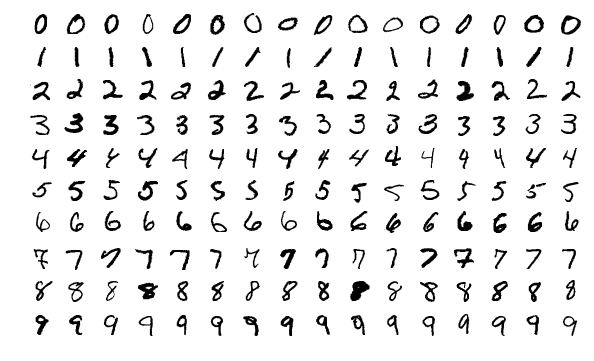
\includegraphics[width=\textwidth]{mnist} \\[5mm]
            \uncover<.->{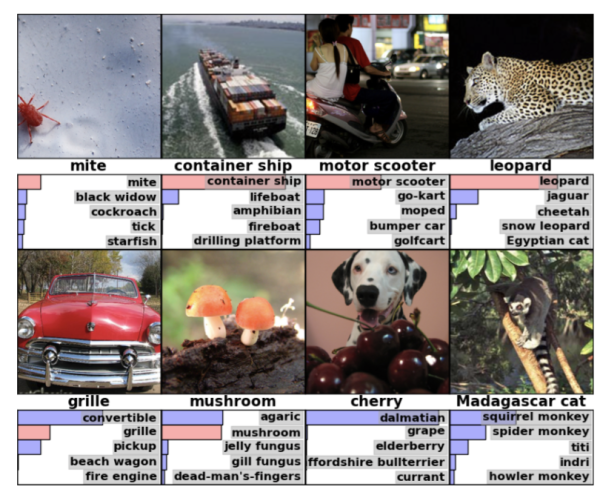
\includegraphics[width=\textwidth]{imagenet}}
        \end{column}
    \end{columns}
\end{frame}

\begin{frame}
    \frametitle{CNN architectures that authors expect you to know}

    \begin{itemize}
        \item LeNet \citep{LeCunIEEE98}
        \item AlexNet \citep{KrizhevskyNIPS12}
        \item VGGNet \citep{Simonyan14}
        \item GoogLeNet/Inception \citep{SzegedyIEEECVPR15}
        \item ResNet \citep{He15b}
    \end{itemize}
\end{frame}

%%% Local Variables:
%%% mode: latex
%%% TeX-master: "../nn"
%%% End:


%%% Local Variables:
%%% mode: latex
%%% TeX-master: "../nn"
%%% End:

% General advice: use GPUs; start small; # parameters vs # data; halving width; normalize data; dropout
% End-to-end.
% Obsolete papers.
% float32.

\footnotesize

\begin{frame}[allowframebreaks]{References}
    \bibliography{nn}
\end{frame}

%%% Local Variables:
%%% mode: latex
%%% TeX-master: "../nn"
%%% End:


\end{document}

%%% Local Variables:
%%% mode: latex
%%% TeX-master: t
%%% End:
